 
%%%%%%%%%%%%%%%%%%%%%%%%%%%%%%%%%%%%%%%%%%%%%%%%%%%%%%%%%%%%
%%% Document created by Yuri Gelsleichter for RBCS,      %%%
%%% with figures and tables automated at end,            %%%    
%%% and references adjusted according journal standards. %%%
%%% April 2022.                                          %%%
%%%                                                      %%%
%%% Journal guidelines:                                  %%%    
%%% https://www.rbcsjournal.org/instructions-to-authors/ %%%
%%%                                                      %%%
%%% if needed convert to word with                       %%%
%%% https://www.adobe.com/br/acrobat/online/             %%%
%%%%%%%%%%%%%%%%%%%%%%%%%%%%%%%%%%%%%%%%%%%%%%%%%%%%%%%%%%%%
%%% Select and run the "Title_page"

\documentclass[a4paper,12pt,twoside]{article}
\usepackage[left=2cm,right=2cm,top=2cm,bottom=3cm]{geometry}
\usepackage{natbib}                         % for Vancouver reference
\usepackage{graphicx}
\usepackage{lineno,hyperref}
\usepackage{ragged2e}                       % for left alignment
\usepackage{caption}                        % for caption in long table
\usepackage{threeparttable}                 % foot note on tables
\usepackage{longtable}                      % to several pages tables (long tables)
\usepackage{subcaption}                     % subfigures
\usepackage{threeparttablex}                % for "ThreePartTable" environment
\usepackage{booktabs}                       % for well-spaced horizontal rules
%\usepackage{amsmath}                        % for equation numbering
\usepackage{mathtools}                      % loads »amsmath«


%%%%%%%%%%%%%%%%%%%%%%%%%%%%%%%% place all figures and tables at end of document
\usepackage[markers,nolists]{endfloat}
\renewcommand{\efloatseparator}{\mbox{}} % allows tables to share a page
% comment because it was called above \usepackage{longtable,threeparttable,booktabs,endfloat}
\usepackage{endfloat} 
\DeclareDelayedFloatFlavour*{longtable}{table}
\DeclareDelayedFloatFlavour{threeparttable}{table}
\usepackage{float}
% source: https://tex.stackexchange.com/questions/340918/how-to-set-the-options-for-the-endfloat-package-when-you-have-to-put-several-pa
%%%%%%%%%%%%%%%%%%%%%%%%%%%%%%%%%%%%%%%%%%%%%%%%%%%%%%%%%%%%%%%%%%%%%%%%%%%%%%%

%%%%%%%%%%%%%%%%%%%%%%%%%%%%%%%%%%%%%%%%%%%%%%%%%%%%%%%%%%%%%%%%%%%%%%%%%%%%%%%
%%% Equation customization: https://tex.stackexchange.com/a/377469/223315
% \newtagform{Alph}[\renewcommand{\theequation}{(\arabic{chapter}.\arabic{section})(\roman{equation})}]{}{}
% \usetagform{Alph}
% \renewcommand{\theequation}{(\arabic{chapter}.\arabic{section})(\roman{equation})}
\newtagform{Alph}[\renewcommand{\theequation}{Eq. \arabic{equation}}]{}{}
\usetagform{Alph}
\renewcommand{\theequation}{\arabic{equation}}
%%%%%%%%%%%%%%%%%%%%%%%%%%%%%%%%%%%%%%%%%%%%%%%%%%%%%%%%%%%%%%%%%%%%%%%%%%%%%%%

\renewcommand{\bibname}{References} % change from "bibliography" to "references"
\linespread{1.25} % correspond to line space 1.5 in word


%%%%%%%%%%%%%%%%%%%%%%%%%%%%%%%%%%%%%%%%%%%%%%%%%%%%%%
%%%%%%%%%%%%%%%%%%%%%%% Article start here
%%%%%%%%%%%%%%%%%%%%%%%%%%%%%%%%%%%%%%%%%%%%%%%%%%%%%%

\begin{document}
\raggedright % for left alignment


\section*{Study Title}

\section*{Highlights}
\begin{itemize}
\item Highlight 1
\item Highlight 2
\item Highlight 3
\end{itemize}

%\modulolinenumbers[5] % for number lines by 5 


\section*{Abstract}
Aside of a template for RBCS, you can find basic LaTex instructions in the document. (Place your abstract here).

\vspace{0.5cm}

\textbf{Keywords:} Keyword1; Keyword2; Keyword3; Keyword4; Keyword5


%\linenumbers %%% uncomment for add linenumbers

%%%%%%%%%%%%%%%%%%%%%%%%%%%%%%%%%%%%%%%%%%
\section{Introduction}

See the \href{https://www.rbcsjournal.org/instructions-to-authors/}{Journal guidelines}.

Your introduction goes here! Simply start writing your document and use the Recompile button to view the updated PDF preview. Examples of commonly used commands and features are listed below, to help you get started.

Once you're familiar with the editor, you can find various project setting in the Overleaf menu, accessed via the button in the very top left of the editor. To view tutorials, user guides, and further documentation, please visit our \href{https://www.overleaf.com/learn}{help library}, or head to our plans page to \href{https://www.overleaf.com/user/subscription/plans}{choose your plan}.

\section{Some examples to get started}

\subsection{How to create Sections and Subsections}

Simply use the section and subsection commands, as in this example document! With Overleaf, all the formatting and numbering is handled automatically according to the template you've chosen. If you're using Rich Text mode, you can also create new section and subsections via the buttons in the editor toolbar.

\subsection{How to include Figures}

First you have to upload the image file from your computer using the upload link in the file-tree menu. Then use the includegraphics command to include it in your document. Use the figure environment and the caption command to add a number and a caption to your figure. See the code for Figure \ref{fig:sample01} in this section for an example.

\begin{figure}
\centering
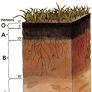
\includegraphics[width=3.5cm]{Figures/Soil_samples/soil_p_1jpg}
\caption{Soil profile.}
\label{fig:sample01}
\end{figure}

Note that your figure will automatically be placed in the most appropriate place for it, given the surrounding text and taking into account other figures or tables that may be close by. You can find out more about adding images to your documents in this help article on \href{https://www.overleaf.com/learn/how-to/Including_images_on_Overleaf}{including images on Overleaf}.
See the Figure \ref{fig:soil_samples} with subfigure.

\begin{figure}
     \centering
     \begin{subfigure}[b]{0.3\textwidth}
         \centering
         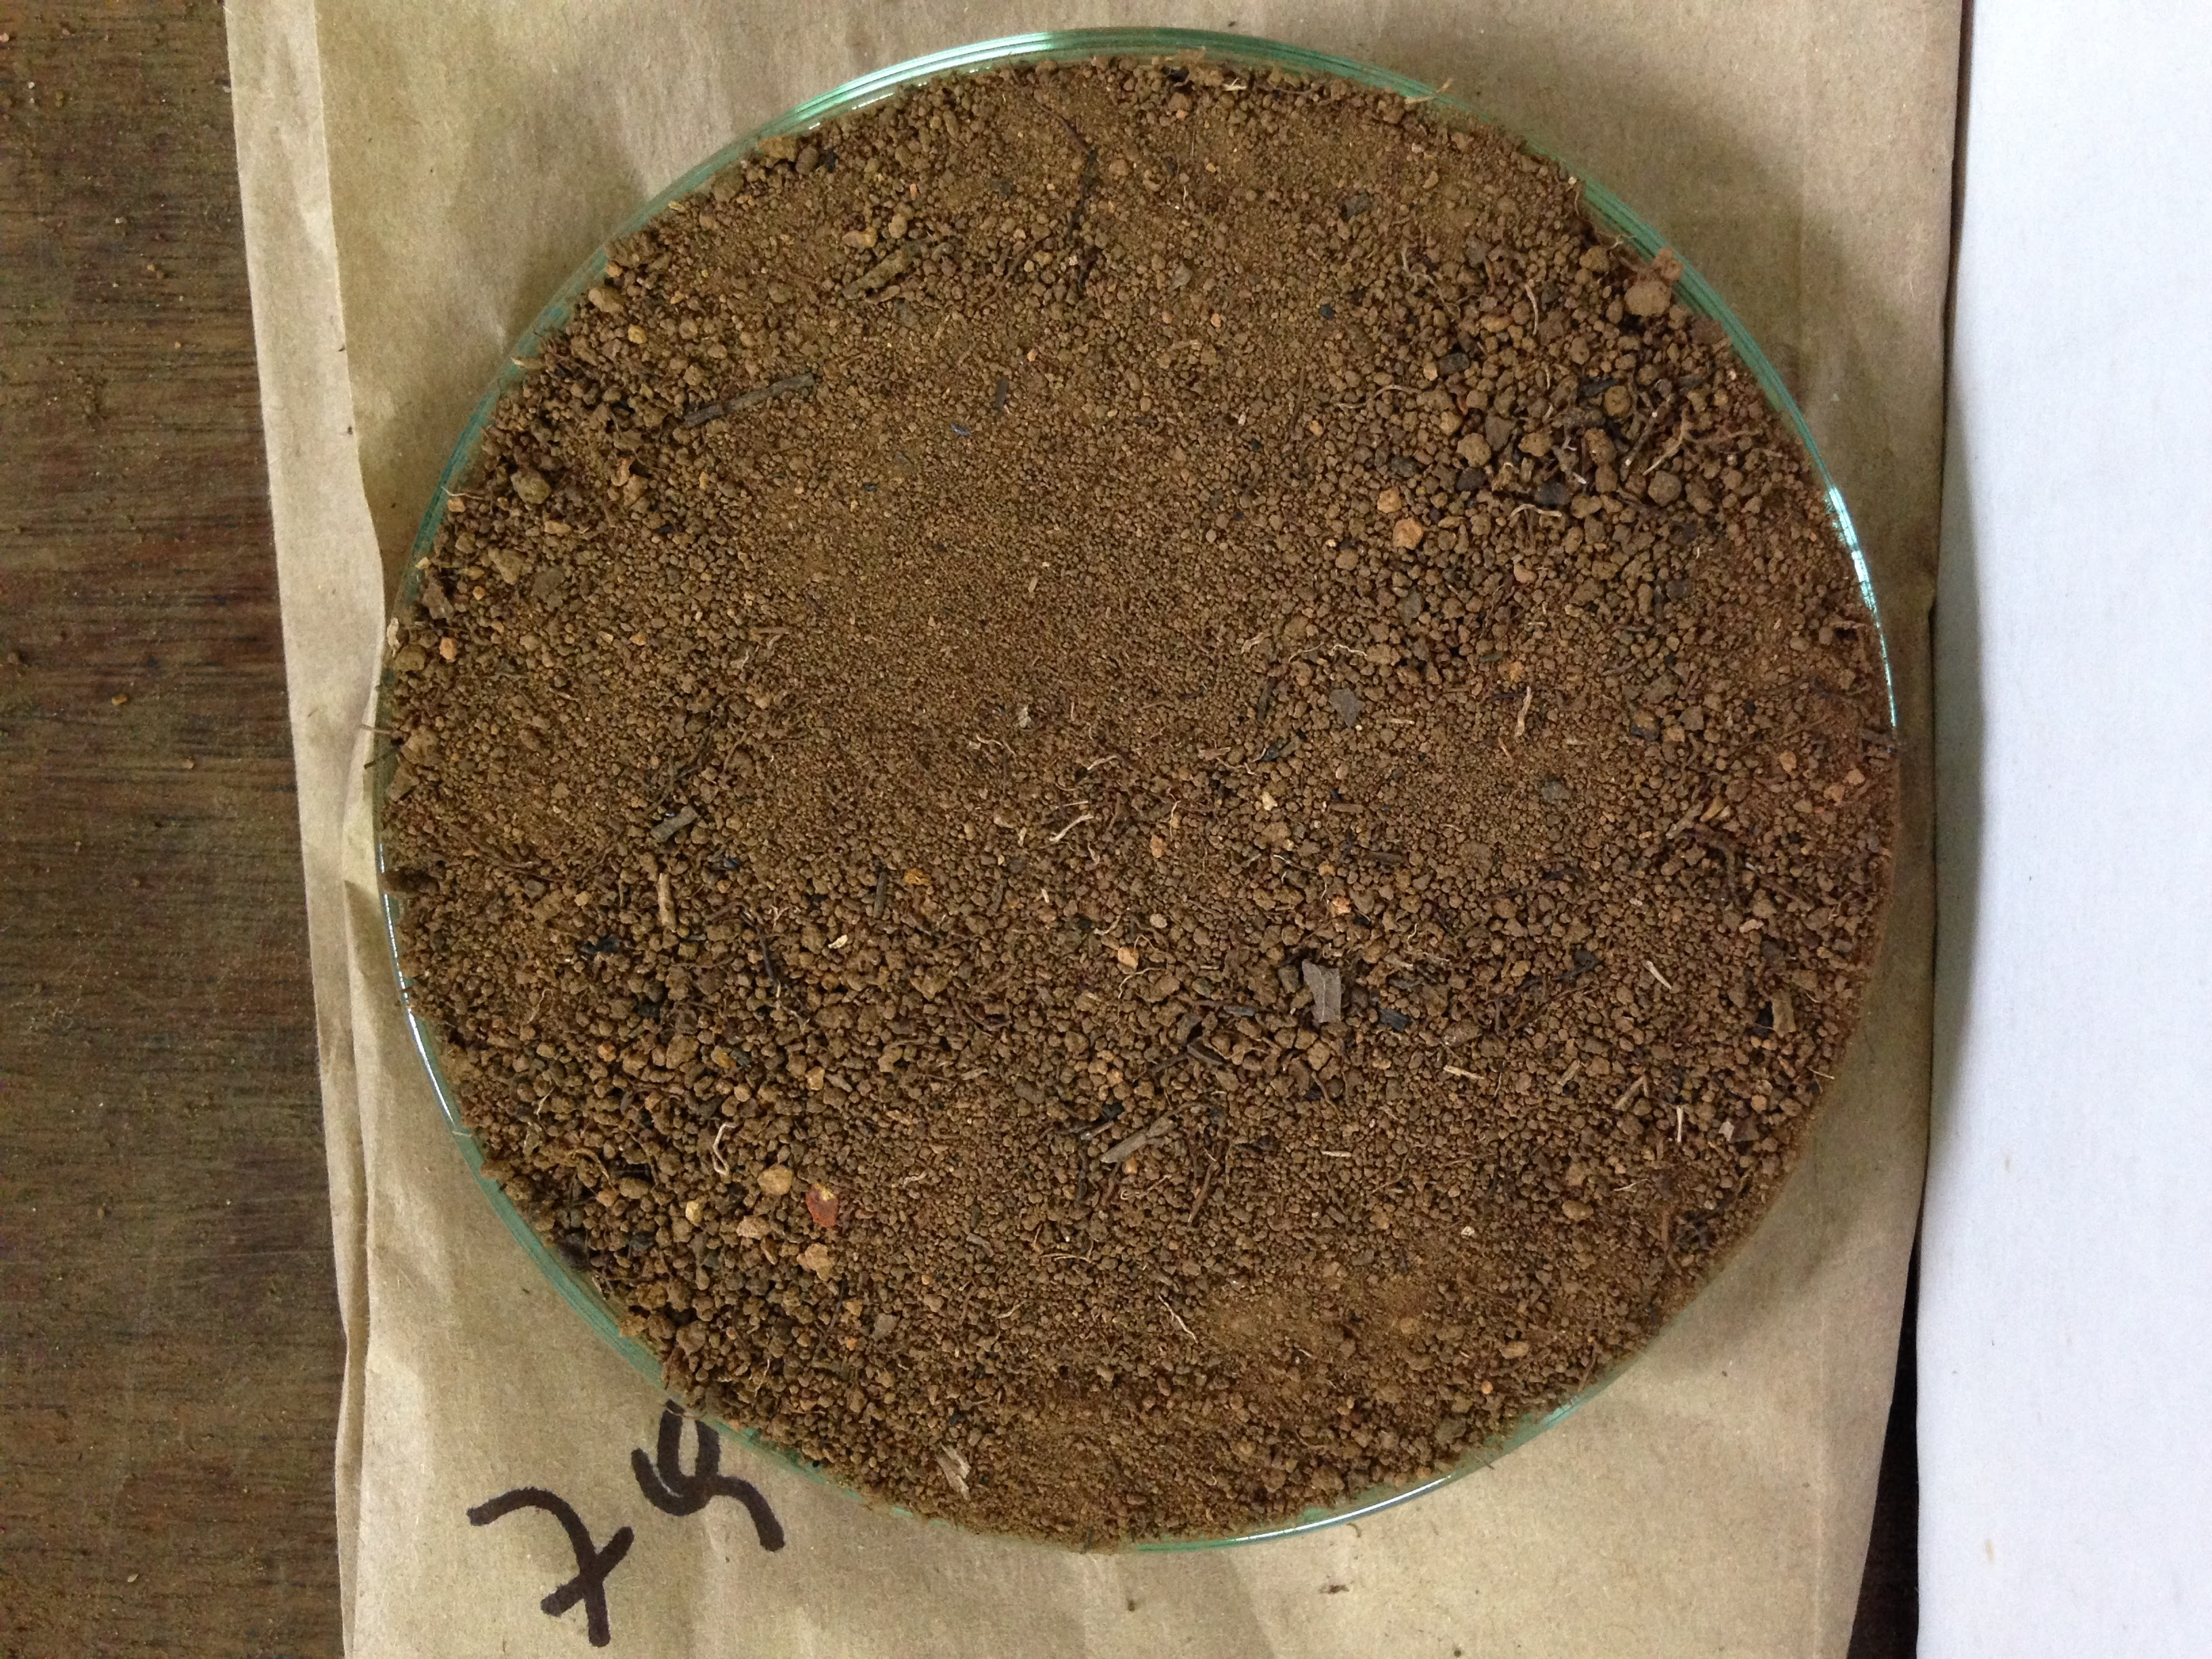
\includegraphics[width=4.5cm]{Figures/Soil_samples/79_O_1}
         \caption{Sample 1}
         \label{fig:horiz1}
     \end{subfigure}
     \hfill
     \begin{subfigure}[b]{0.3\textwidth}
         \centering
         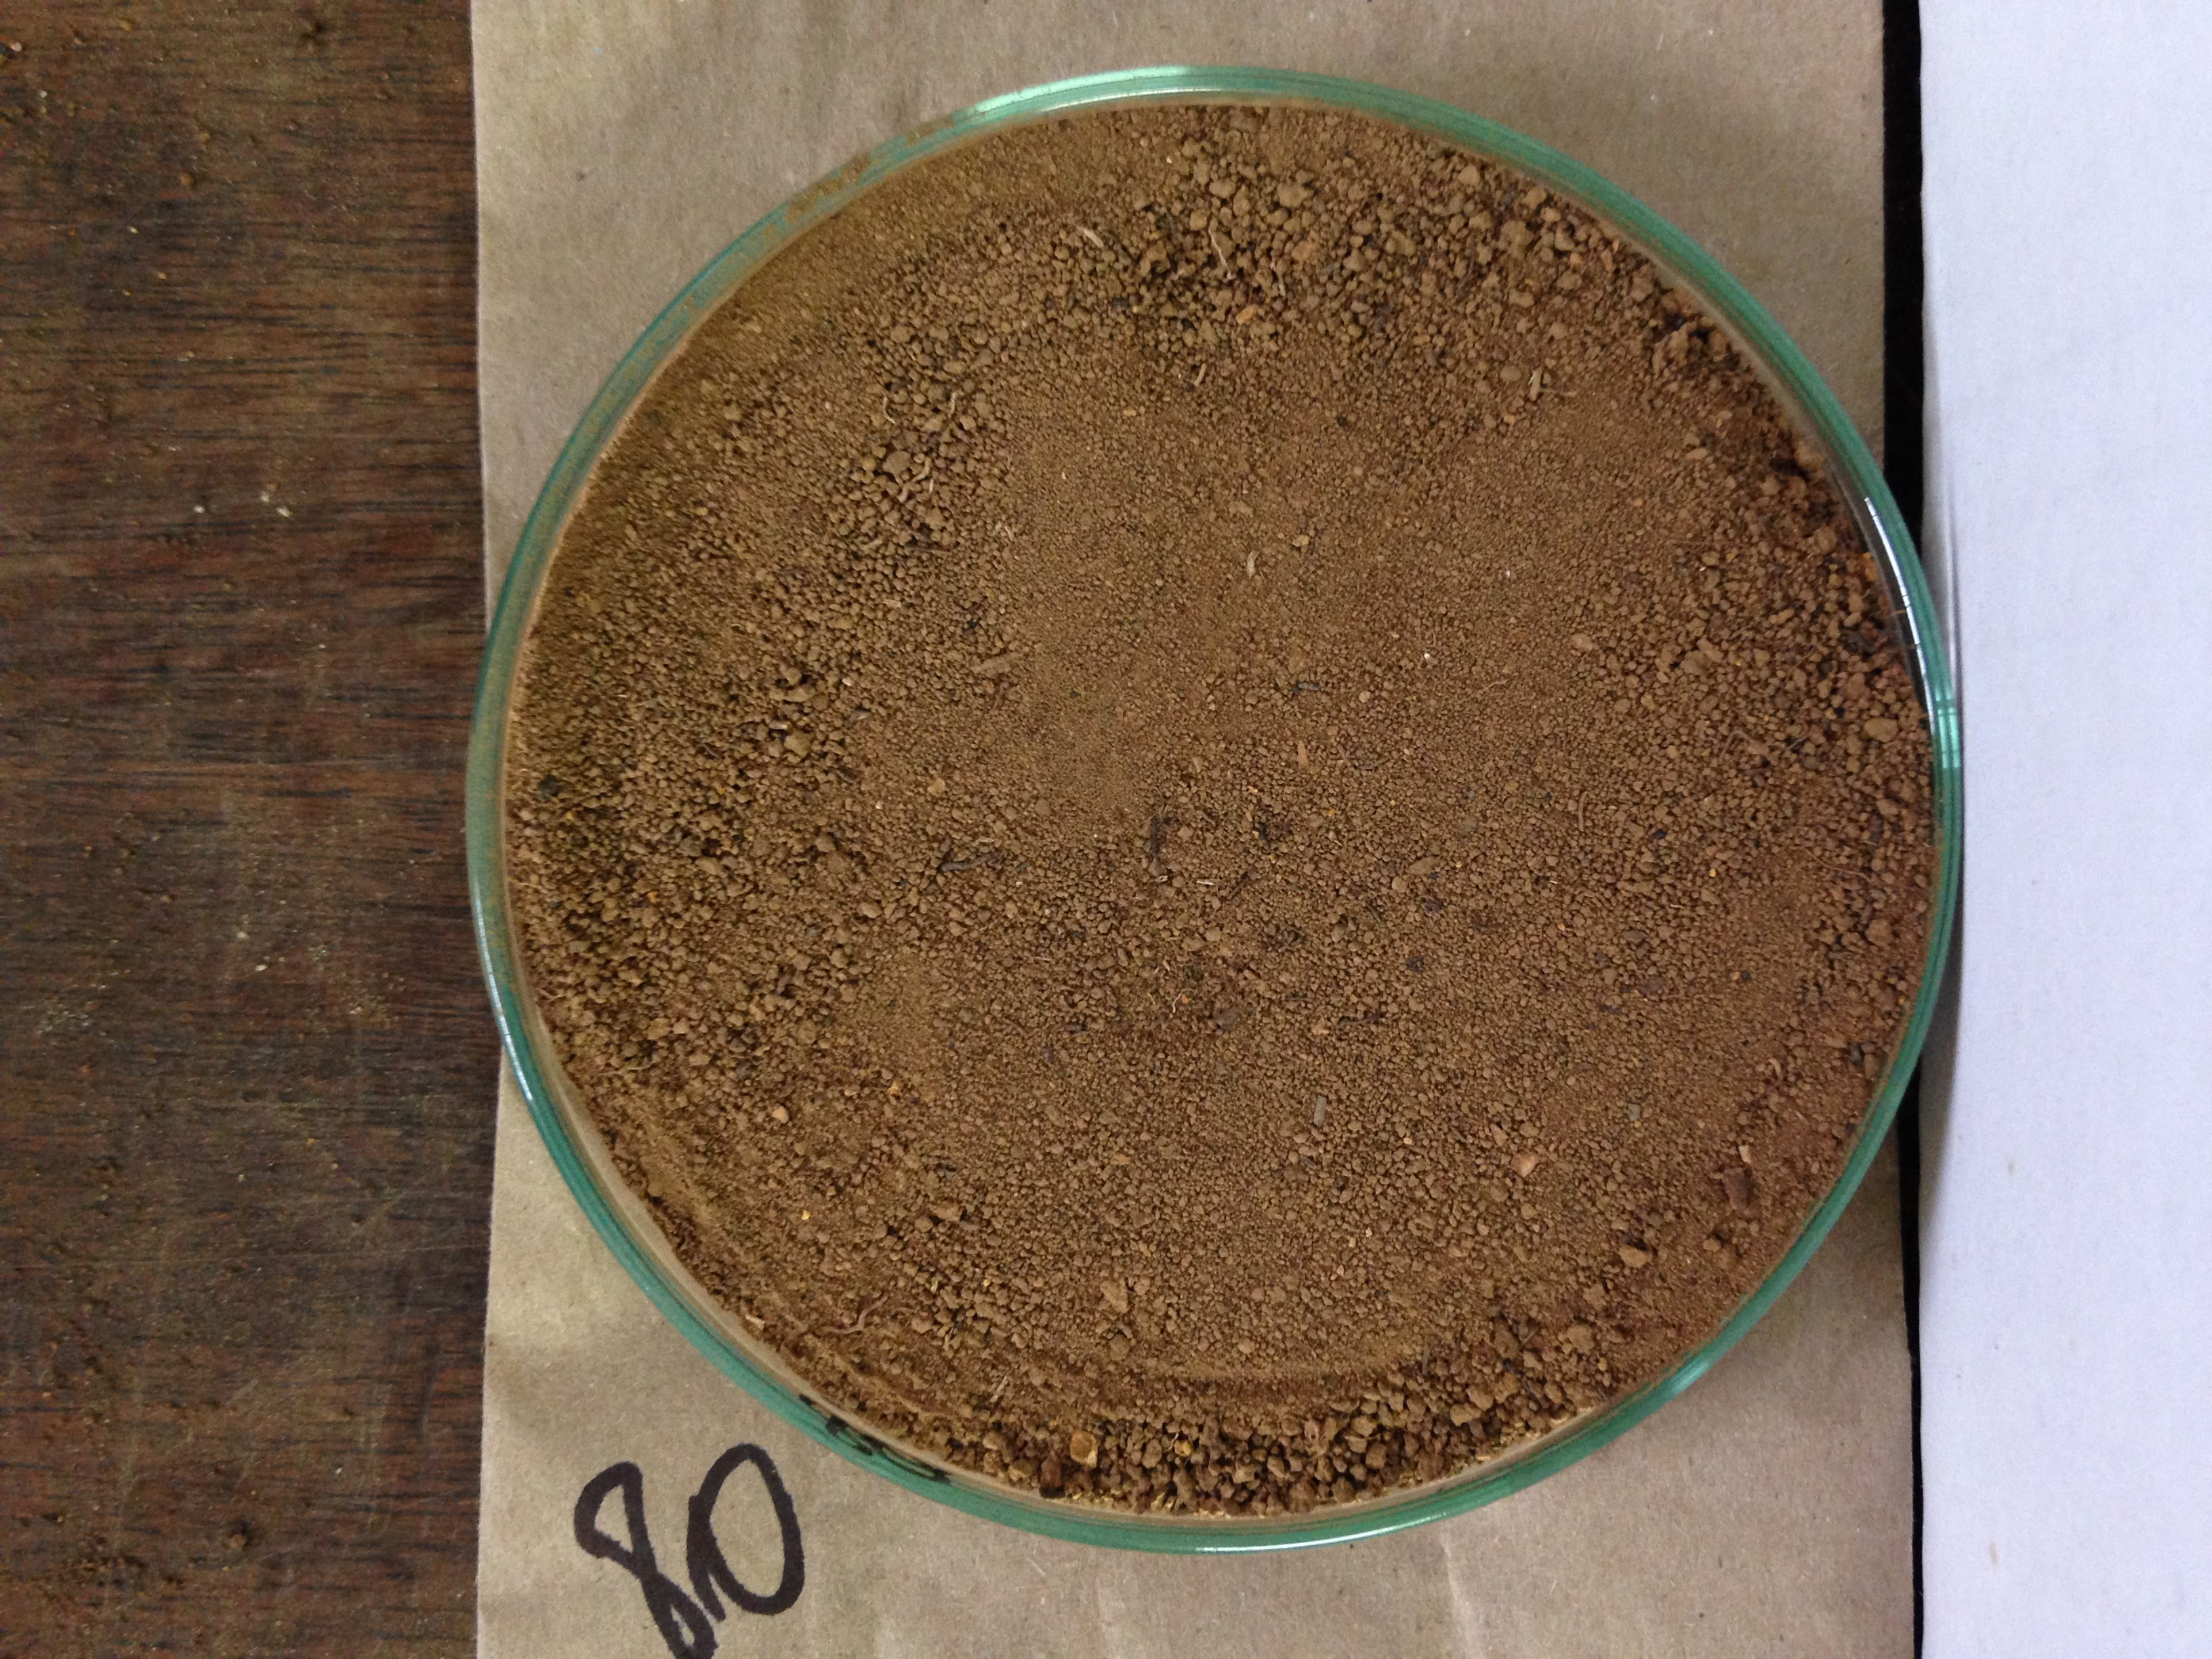
\includegraphics[width=4.5cm]{Figures/Soil_samples/80_OB_2}
         \caption{Sample 2}
         \label{fig:horiz2}
     \end{subfigure}
     \hfill
     \begin{subfigure}[b]{0.3\textwidth}
         \centering
         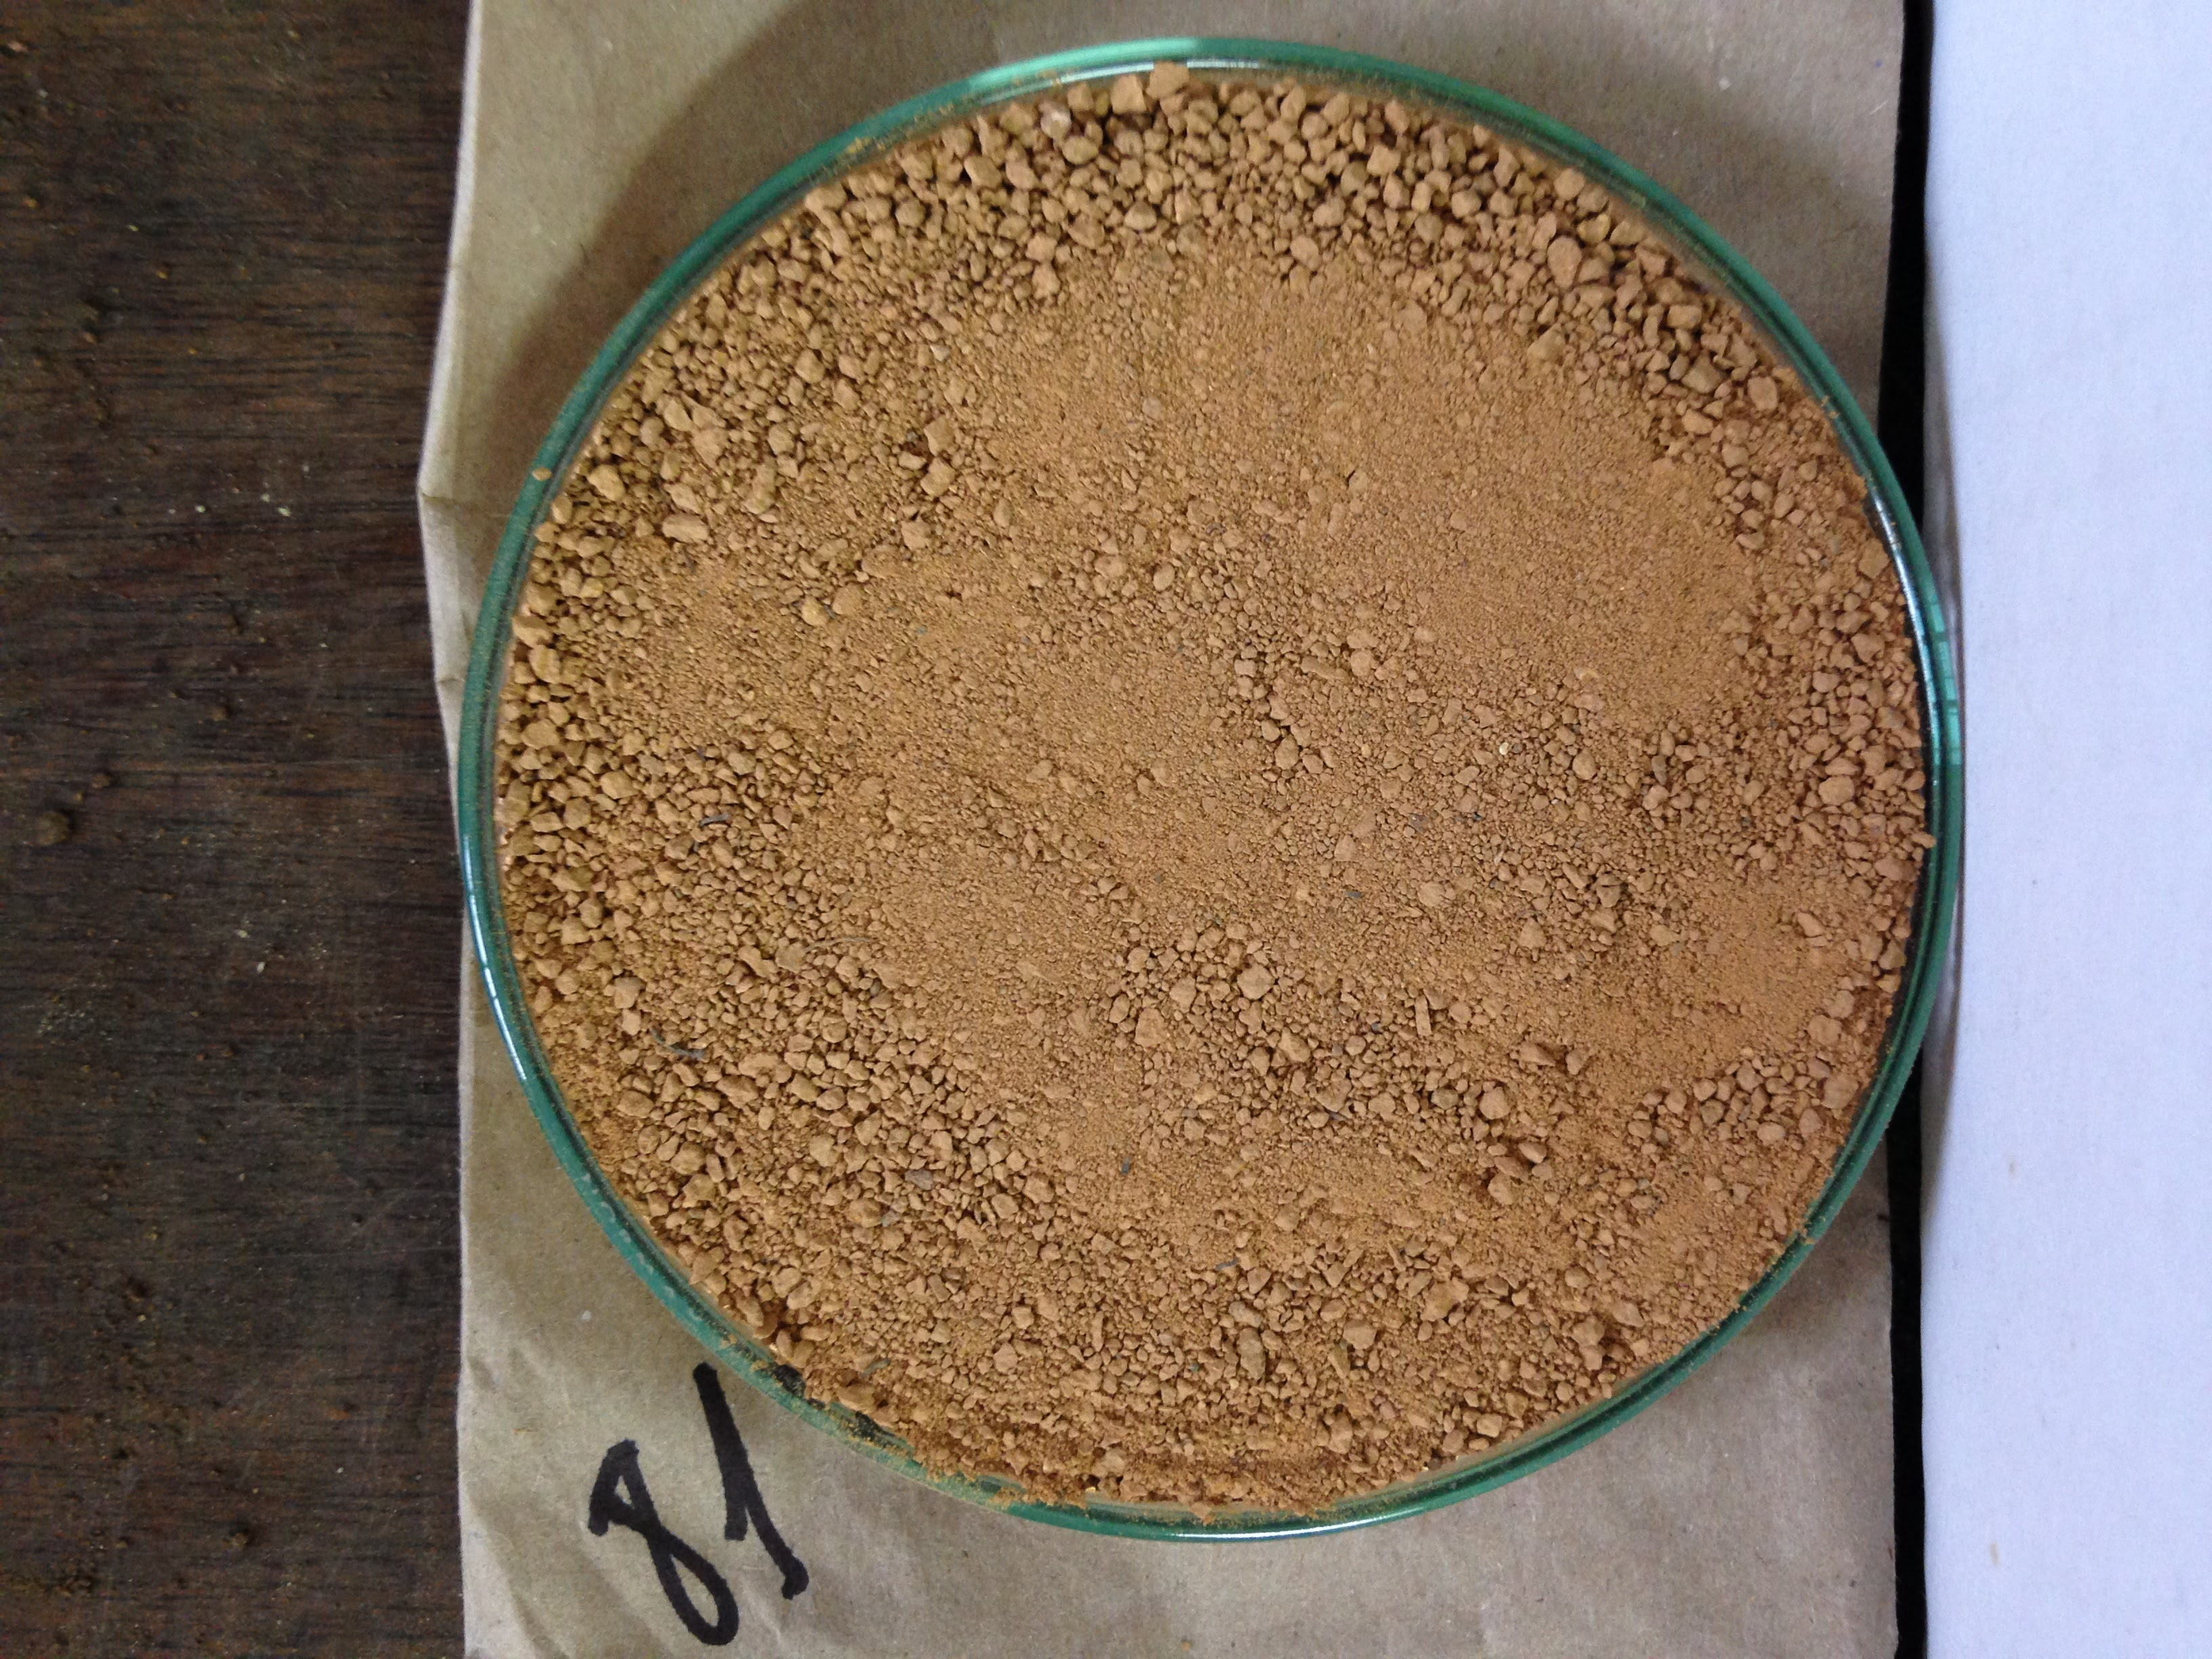
\includegraphics[width=4.5cm]{Figures/Soil_samples/81_Bi1_3}
         \caption{Sample 3}
         \label{fig:horiz3}
     \end{subfigure}
        \caption{Three Soil samples in subfigure}
        \label{fig:soil_samples}
\end{figure}


\subsection{How to add Tables}

Use the table and tabular environments for basic tables see Table \ref{tab:test} and \ref{tab:test2}, for example. For more information, please see this help article on \href{https://www.overleaf.com/learn/latex/tables}{tables}. 

\begin{table}[h]
\centering
\caption{Table to test captions and labels.}
\label{tab:test}
\begin{tabular}{c c c c} 
    \hline
    Col1 & Col2 & Col2 & Col3 \\ 
    \hline
    1 & 6 & 87837 & 787 \\ 
    2 & 7 & 78 & 5415 \\
    3 & 545 & 778 & 7507 \\
    4 & 545 & 18744 & 7560 \\
    5 & 88 & 788 & 6344 \\ 
    \hline
\end{tabular}
\end{table}

\begin{table}[h]
	%\footnotesize % ao inves de fonte menor, foi utilizada a redução de espaço para acampanhar a tabela seguinte
	%\renewcommand{\tabcolsep}{1pt} %%% no caso de usar negrito
	\renewcommand{\tabcolsep}{2.6pt} %%% redução de espaço entre as colunas
	%\begin{threeparttable}[h]
	\centering
	\caption{Table description.}
	\label{tab:test2}
	\vspace{0cm}
	\begin{tabular}{ l c c c c c c c }
		\toprule
		%\textbf{Preprocessing} & \textbf{Model} & \textbf{Soil property*} & \textbf{R$^2$} & \textbf{MSE} & \textbf{RMSE} & \textbf{bias} & \textbf{RPD} \\ 
		Preprocessing     & Model & Soil property* & R$^2$ & MSE & RMSE & bias & RPD \\ 
		\midrule
		Process 123       & rf   & Al & 0.12 & 1.2 & 0.3 & 0.002 & 1.5 \\
		Process 123       & cb   & H  & 0.12 & 1.2 & 0.3 & 0.002 & 1.5 \\
		Process 123       & rf   & K  & 0.12 & 1.2 & 0.3 & 0.002 & 1.5 \\
		Process 123       & rf   & Mg & 0.12 & 1.2 & 0.3 & 0.002 & 1.5 \\
		Process 123       & plsr & N  & 0.12 & 1.2 & 0.3 & 0.002 & 2.5 \\
		Process 123       & rf   & P  & 0.12 & 1.2 & 7.3 & 0.002 & 1.5 \\
		Process 123       & rf   & pH & 0.12 & 1.2 & 0.3 & 0.002 & 1.5 \\
		Process 123       & cb   & TC & 0.12 & 1.2 & 1.3 & 0.002 & 2.5 \\
		\bottomrule
	\end{tabular}
	%\begin{tablenotes}[para, flushleft]
	\begin{tablenotes}
	\footnotesize
	\item[*] Note 1, description...
	%\item[**] note 2
	\end{tablenotes}
	%\end{threeparttable}
	%\medskip
	%\begin{minipage}{\linewidth}\footnotesize
	%	*Note 1, description...
	%\end{minipage}
\end{table}


For long table see the example \ref{tab:all_pre_treatment}.

%%%%%%%%%%%%%%%%%%%%%%%%%%%%%%%%%%%%%%%%%%%%%%%%%%%%%%%%%%%%%%%%%%%%%%%%%%%%%%%%%%%%%%%%%%%%%%
%%% tabela longa: https://tex.stackexchange.com/questions/209841/long-table-with-tablenote
%%% nota alinhada https://tex.stackexchange.com/questions/19991/align-note-below-table
%%%%%%%%%%%%%%%%%%%%%%%%%%%%%%%%%%%%%%%%%%%%%%%%%%%%%%%%%%%%%%%%%%%%%%%%%%%%%%%%%%%%%%%%%%%%%%

%\begin{center}
\begin{ThreePartTable}
	\begin{TableNotes}[para,flushleft] 
		\footnotesize
		%\note The description...
		\item [] note description on the bottom of the table.
		%\item [b] Partial least squares regression
	\end{TableNotes}
	\renewcommand{\tabcolsep}{3.5pt} %%% redução de espaço entre as colunas
	\begin{longtable}[c]{ l c c c c c c c }
		\caption{Description on the top of table.} \label{tab:all_pre_treatment} \\
		%%% negrito
		%%% \multicolumn{1}{l}{\textbf{Preprocessing}} & \multicolumn{1}{c}{\textbf{Model}} & \multicolumn{1}{c}{\textbf{Soil property}} & \multicolumn{1}{c}{\textbf{R$^2$}} & \multicolumn{1}{c}{\textbf{MSE}} & \multicolumn{1}{c}{\textbf{RMSE}} & \multicolumn{1}{c}{\textbf{bias}} & \multicolumn{1}{c}{\textbf{RPD}} \\ \hline
		\toprule
		%%% normal
		\multicolumn{1}{l}{Preprocessing} & \multicolumn{1}{c}{Model} & \multicolumn{1}{c}{Soil property} & \multicolumn{1}{c}{R$^2$} & \multicolumn{1}{c}{MSE} & \multicolumn{1}{c}{RMSE} & \multicolumn{1}{c}{bias} & \multicolumn{1}{c}{RPD} \\
		\midrule
		\endfirsthead
		%{\tablename\ \thetable{} -- continued from previous page} \\
		\captionsetup{justification=raggedright,singlelinecheck=false, skip=0pt} %%% opcional font=small
		\caption*{\tablename\ \thetable{} -- continued from previous page}\\
		\toprule
		\multicolumn{1}{l}{Preprocessing} & \multicolumn{1}{c}{Model} & \multicolumn{1}{c}{Soil property} & \multicolumn{1}{c}{R$^2$} & \multicolumn{1}{c}{MSE} & \multicolumn{1}{c}{RMSE} & \multicolumn{1}{c}{bias} & \multicolumn{1}{c}{RPD} \\
		\midrule
		\endhead
		\bottomrule
		\captionsetup{justification=raggedleft,singlelinecheck=false, skip=0pt} %%% opcional font=small
		\caption*{\tablename\ \thetable{} -- continued on the next page}\\
		\endfoot
		\bottomrule
		\insertTableNotes  % tell LaTeX where to insert the contents of ``TableNotes"
		\endlastfoot
		Process 123                & cb   & TC & 0.1 & 3.2 & 1.3 & -0.1 & 2.27 \\
		Process 123                & rf   & TC & 0.1 & 4.2 & 2.3 & -0.1 & 2.2  \\
		Process 123                & rf   & TC & 0.1 & 4.2 & 2.3 & -0.1 & 2.29 \\
		Process 123                & rf   & TC & 0.1 & 4.2 & 2.3 & -0.1 & 2.27 \\
		Process 123                & rf   & TC & 0.1 & 4.2 & 2.3 & -0.1 & 2.24 \\
		Process 123                & rf   & TC & 0.1 & 4.2 & 2.3 & -0.1 & 2.22 \\
		Process 123                & cb   & TC & 0.1 & 4.2 & 2.3 & -0.1 & 2.22 \\
		Process 123                & rf   & TC & 0.1 & 5.2 & 2.3 & -0.1 & 2.29 \\
		Process 123                & rf   & TC & 0.1 & 5.2 & 2.3 & -0.1 & 2.29 \\
		Process 123                & plsr & TC & 0.1 & 4.2 & 2.3 & -0.1 & 2.29 \\
		Process 123                & cb   & TC & 0.1 & 5.2 & 2.3 & -0.1 & 2.27 \\
		Process 123                & rf   & TC & 0.1 & 5.2 & 2.3 & -0.1 & 2.22 \\
		Process 123                & cb   & TC & 0.1 & 5.2 & 2.3 & -0.1 & 2.26 \\
		Process 123                & cb   & TC & 0.1 & 5.2 & 2.3 & -0.1 & 2.28 \\
		Process 123                & cb   & TC & 0.1 & 6.2 & 2.3 & -0.1 & 2.28 \\
		Process 123                & plsr & N  & 0.1 & 0.2 & 0.3 & -0.1 & 2.29 \\
		Process 123                & rf   & N  & 0.1 & 0.2 & 0.3 & -0.1 & 2.26 \\
		Process 123                & rf   & N  & 0.1 & 0.2 & 0.3 & -0.1 & 2.26 \\
		Process 123                & plsr & N  & 0.1 & 0.2 & 0.3 & -0.1 & 2.2  \\
		Process 123                & rf   & N  & 0.1 & 0.2 & 0.3 & -0.1 & 2.22 \\
		Process 123                & rf   & N  & 0.1 & 0.2 & 0.3 & -0.1 & 2.2  \\
		Process 123                & rf   & N  & 0.1 & 0.2 & 0.3 & -0.1 & 2.21 \\
		Process 123                & rf   & N  & 0.1 & 0.2 & 0.3 & -0.1 & 2.25 \\
		Process 123                & rf   & N  & 0.1 & 0.2 & 0.3 & -0.1 & 2.28 \\
		Process 123                & cb   & N  & 0.1 & 0.2 & 0.3 & -0.1 & 2.25 \\
		Process 123                & rf   & N  & 0.1 & 0.2 & 0.3 & -0.1 & 2.26 \\
		Process 123                & cb   & N  & 0.1 & 0.2 & 0.3 & -0.1 & 2.21 \\
		Process 123                & cb   & N  & 0.1 & 0.2 & 0.3 & -0.1 & 2.22 \\
		Process 123                & cb   & N  & 0.1 & 0.2 & 0.3 & -0.1 & 2.25 \\
		Process 123                & cb   & N  & 0.1 & 0.2 & 0.3 & -0.1 & 1.2  \\
		Process 123                & rf   & Al & 0.1 & 0.2 & 0.3 & -0.1 & 1.21 \\
		Process 123                & rf   & Al & 0.1 & 0.2 & 0.3 & -0.1 & 1.27 \\
		Process 123                & rf   & Al & 0.1 & 0.2 & 0.3 & -0.1 & 1.29 \\
		Process 123                & cb   & Al & 0.1 & 0.2 & 0.3 & -0.1 & 1.24 \\
		Process 123                & rf   & Al & 0.1 & 0.2 & 0.3 & -0.1 & 1.2  \\
		Process 123                & rf   & Al & 0.1 & 0.2 & 0.3 & -0.1 & 1.26 \\
		Process 123                & rf   & Al & 0.1 & 1.2 & 0.3 & -0.1 & 1.25 \\
		Process 123                & rf   & Al & 0.1 & 1.2 & 1.3 & -0.1 & 1.29 \\
		Process 123                & cb   & Al & 0.1 & 1.2 & 1.3 & -0.1 & 1.25 \\
		Process 123                & cb   & Al & 0.1 & 1.2 & 1.3 & -0.1 & 1.21 \\
		Process 123                & cb   & Al & 0.1 & 1.2 & 1.3 & -0.1 & 1.29 \\
		Process 123                & rf   & Al & 0.1 & 1.2 & 1.3 & -0.1 & 1.22 \\
		Process 123                & cb   & Al & 0.1 & 1.2 & 1.3 & -0.1 & 1.29 \\
		Process 123                & cb   & Al & 0.1 & 1.2 & 1.3 & -0.1 & 1.25 \\
		Process 123                & rf   & Al & 0.1 & 1.2 & 1.3 & -0.1 & 1.23 \\
		Process 123                & rf   & pH & 0.1 & 0.2 & 0.3 & -0.1 & 1.26 \\
		Process 123                & rf   & pH & 0.1 & 0.2 & 0.3 & -0.1 & 1.28 \\
		Process 123                & rf   & pH & 0.1 & 0.2 & 0.3 & -0.1 & 1.27 \\
		Process 123                & rf   & pH & 0.1 & 0.2 & 0.3 & -0.1 & 1.24 \\
		Process 123                & rf   & pH & 0.1 & 0.2 & 0.3 & -0.1 & 1.2  \\
		Process 123                & rf   & pH & 0.1 & 0.2 & 0.3 & -0.1 & 1.25 \\
		Process 123                & rf   & pH & 0.1 & 0.2 & 0.3 & -0.1 & 1.29 \\
		Process 123                & cb   & pH & 0.1 & 0.2 & 0.3 & -0.1 & 1.2  \\
		Process 123                & cb   & pH & 0.1 & 0.2 & 0.3 & -0.1 & 1.22 \\
		Process 123                & rf   & pH & 0.1 & 0.2 & 0.3 & -0.1 & 1.23 \\
		Process 123                & cb   & pH & 0.1 & 0.2 & 0.3 & -0.1 & 1.25 \\
		Process 123                & cb   & pH & 0.1 & 0.2 & 0.3 & -0.1 & 1.27 \\
		Process 123                & rf   & pH & 0.1 & 0.2 & 0.3 & -0.1 & 1.22 \\
		no preprocessing           & rf   & pH & 0.1 & 0.2 & 0.3 & -0.1 & 1.2  \\
		no preprocessing           & rf   & pH & 0.1 & 0.2 & 0.3 & -0.1 & 1.27 \\
	\end{longtable}
\end{ThreePartTable}
%\end{center}

%%%%%%%%%%%%%%%%%%%%%%%%%%%%%%%%%%%%%%%%%%%%%%%%%%%%%%%%%%%%%%%%%%%%
%%% End longtable
%%%%%%%%%%%%%%%%%%%%%%%%%%%%%%%%%%%%%%%%%%%%%%%%%%%%%%%%%%%%%%%%%%%%


\subsection{How to add Comments and Track Changes}

Comments can be added to your project by highlighting some text and clicking ``Add comment'' in the top right of the editor pane. To view existing comments, click on the Review menu in the toolbar above. To reply to a comment, click on the Reply button in the lower right corner of the comment. You can close the Review pane by clicking its name on the toolbar when you're done reviewing for the time being.

Track changes are available on all our \href{https://www.overleaf.com/user/subscription/plans}{premium plans}, and can be toggled on or off using the option at the top of the Review pane. Track changes allow you to keep track of every change made to the document, along with the person making the change. 

\subsection{How to add Lists}

You can make lists with automatic numbering \dots

\begin{enumerate}
\item Like this,
\item and like this.
\end{enumerate}
\dots or bullet points \dots
\begin{itemize}
\item Like this,
\item and like this.
\end{itemize}


\subsection{Equations}

Equations should be cited along the text as “equation 1”, using a lowercase letter; or highlighted in parenthesis (Equation 1). Equations should be numbered consecutively as Eq.1, Eq. 2, Eq. 3, etc. at the right-hand side.

The well known Pythagorean theorem that can be ref as equation \ref{eq:equation1} or (Equation \ref{eq:equation1}), was proved to be invalid for other exponents. 
Meaning the next equation has no integer solutions:

\begin{equation}
x^n + y^n = z^n
\label{eq:equation1}
\end{equation}

See also the equation \ref{eq:equation2} below:

\begin{equation}
    \log \mu_{ijk}= \lambda + \lambda_i ^I + \lambda_j ^J+\lambda_k ^K+\lambda_{ij} ^{IJ}+\lambda_{ik} ^{IK}+\lambda_{jk} ^{JK}+\lambda_{ijk} ^{IJK} 
    \label{eq:equation2}
\end{equation}  


\subsection{How to change the margins and paper size}

Usually the template you're using will have the page margins and paper size set correctly for that use-case. For example, if you're using a journal article template provided by the journal publisher, that template will be formatted according to their requirements. In these cases, it's best not to alter the margins directly.

If however you're using a more general template, such as this one, and would like to alter the margins, a common way to do so is via the geometry package. You can find the geometry package loaded in the preamble at the top of this example file, and if you'd like to learn more about how to adjust the settings, please visit this help article on \href{https://www.overleaf.com/learn/latex/page_size_and_margins}{page size and margins}.

\subsection{How to change the document language and spell check settings}

Overleaf supports many different languages, including multiple different languages within one document. 

To configure the document language, simply edit the option provided to the babel package in the preamble at the top of this example project. To learn more about the different options, please visit this help article on \href{https://www.overleaf.com/learn/latex/International_language_support}{international language support}.

To change the spell check language, simply open the Overleaf menu at the top left of the editor window, scroll down to the spell check setting, and adjust accordingly.

\subsection{How to add Citations and a References List}

You can simply upload a ".bib" file containing your BibTeX entries, created with a tool such as JabRef, Zotero or Mendeley. You can then cite entries from it, like this: \cite{Bortolotti2006}. Or cite with parenthesis as \citep{Brade1956}.

And multiple author: \cite{Bortolotti2006, Minasny2006}. Or cite with parenthesis as \citep{Brade1956, Bortolotti2006, Minasny2006, Roudier2012}.

See the \href{https://www.rbcsjournal.org/instructions-to-authors/}{Journal guidelines}.

Just remember to specify a bibliography style, as well as the filename of the ".bib". You can find a \href{https://www.overleaf.com/help/97-how-to-include-a-bibliography-using-bibtex}{video tutorial here} to learn more about BibTeX.

If you have an \href{https://www.overleaf.com/user/subscription/plans}{upgraded account}, you can also import your Mendeley or Zotero library directly as a ".bib" file, via the upload menu in the file-tree.

\subsection{Good luck!}

We hope you find Overleaf useful, and do take a look at our \href{https://www.overleaf.com/learn}{help library} for more tutorials and user guides! Please also let us know if you have any feedback using the Contact Us link at the bottom of the Overleaf menu --- or use the contact form at \url{https://www.overleaf.com/contact}.

\section*{Supplementary data}
Supplementary data to this article can be found online at https://doi.org/10.1016/XXX.

% Loading bibliography database
\setlength{\bibhang}{0pt} %%% to aling references to the left: https://tex.stackexchange.com/questions/82731/how-to-align-bibliography-to-the-left
\bibliographystyle{vancouver-authoryear}
\bibliography{references.bib}

%\processdelayedfloats %%% place all figures and tables at end of the document by this command

\end{document}